\documentclass{article}\usepackage[]{graphicx}\usepackage[]{color}
% maxwidth is the original width if it is less than linewidth
% otherwise use linewidth (to make sure the graphics do not exceed the margin)
\makeatletter
\def\maxwidth{ %
  \ifdim\Gin@nat@width>\linewidth
    \linewidth
  \else
    \Gin@nat@width
  \fi
}
\makeatother

\definecolor{fgcolor}{rgb}{0.345, 0.345, 0.345}
\newcommand{\hlnum}[1]{\textcolor[rgb]{0.686,0.059,0.569}{#1}}%
\newcommand{\hlstr}[1]{\textcolor[rgb]{0.192,0.494,0.8}{#1}}%
\newcommand{\hlcom}[1]{\textcolor[rgb]{0.678,0.584,0.686}{\textit{#1}}}%
\newcommand{\hlopt}[1]{\textcolor[rgb]{0,0,0}{#1}}%
\newcommand{\hlstd}[1]{\textcolor[rgb]{0.345,0.345,0.345}{#1}}%
\newcommand{\hlkwa}[1]{\textcolor[rgb]{0.161,0.373,0.58}{\textbf{#1}}}%
\newcommand{\hlkwb}[1]{\textcolor[rgb]{0.69,0.353,0.396}{#1}}%
\newcommand{\hlkwc}[1]{\textcolor[rgb]{0.333,0.667,0.333}{#1}}%
\newcommand{\hlkwd}[1]{\textcolor[rgb]{0.737,0.353,0.396}{\textbf{#1}}}%
\let\hlipl\hlkwb

\usepackage{framed}
\makeatletter
\newenvironment{kframe}{%
 \def\at@end@of@kframe{}%
 \ifinner\ifhmode%
  \def\at@end@of@kframe{\end{minipage}}%
  \begin{minipage}{\columnwidth}%
 \fi\fi%
 \def\FrameCommand##1{\hskip\@totalleftmargin \hskip-\fboxsep
 \colorbox{shadecolor}{##1}\hskip-\fboxsep
     % There is no \\@totalrightmargin, so:
     \hskip-\linewidth \hskip-\@totalleftmargin \hskip\columnwidth}%
 \MakeFramed {\advance\hsize-\width
   \@totalleftmargin\z@ \linewidth\hsize
   \@setminipage}}%
 {\par\unskip\endMakeFramed%
 \at@end@of@kframe}
\makeatother

\definecolor{shadecolor}{rgb}{.97, .97, .97}
\definecolor{messagecolor}{rgb}{0, 0, 0}
\definecolor{warningcolor}{rgb}{1, 0, 1}
\definecolor{errorcolor}{rgb}{1, 0, 0}
\newenvironment{knitrout}{}{} % an empty environment to be redefined in TeX

\usepackage{alltt}
\usepackage{hyperref}

\hypersetup{
    colorlinks=true,
    linkcolor=blue,
    filecolor=magenta,      
    urlcolor=cyan,
}

\usepackage{listings}
\usepackage{color}

\definecolor{dkgreen}{rgb}{0,0.6,0}
\definecolor{gray}{rgb}{0.5,0.5,0.5}
\definecolor{mauve}{rgb}{0.58,0,0.82}

\lstset{frame=tb,
  language=bash,
  aboveskip=3mm,
  belowskip=3mm,
  showstringspaces=false,
  columns=flexible,
  basicstyle={\small\ttfamily},
  numbers=none,
  numberstyle=\tiny\color{gray},
  keywordstyle=\color{blue},
  commentstyle=\color{dkgreen},
  stringstyle=\color{mauve},
  breaklines=true,
  breakatwhitespace=true,
  tabsize=3
}

\author{Anna Burns}
\title{Regional Weather Analysis: Lake County, Illinois}
\IfFileExists{upquote.sty}{\usepackage{upquote}}{}
\begin{document}
\maketitle

I began this project by obtaining data from NOAA's online weather database.  Analyzing the maximum and minimum temperature trends in Lake County, IL contained limited useful information.  As demonstrated in Table 1, while the months of April and August demonstrate a low-significance warming trend in minimum temperatures, and February, September and October demonstrate a warming trend in maximum temperatures (while July actually shows a cooling trend), because our confidence level is 0.05 and we have twelve samples, the likelihood of a Type I error is very high.  There is limited statistical evidence to reject the null hypothesis that there is no significant monthly temperature trends over time.  Therefore, it was necessary to look for other ways that climate change has impacted the Lake County region. 

\begin{table}[ht]
\centering
\begin{tabular}{rlllll}
  \hline
 & Month & Slope TMIN & R\verb|^|2 & Slope TMAX & R\verb|^|2.1 \\ 
  \hline
1 & January & 0.006 NS & 0.003 & 0.0016 NS & 0 \\ 
  2 & February & 0.0182 NS & 0.031 & 0.0182 * & 0.046 \\ 
  3 & March & -0.0034 NS & 0.002 & -0.0067 NS & 0.006 \\ 
  4 & April & 0.0114 * & 0.047 & 0.0027 NS & 0.001 \\ 
  5 & May & 0.0061 NS & 0.01 & -0.0076 NS & 0.011 \\ 
  6 & June & 0.0119 * & 0.049 & -0.0056 NS & 0.011 \\ 
  7 & July & 0.0075 NS & 0.029 & -0.0185 ** & 0.123 \\ 
  8 & August & 0.0145 * & 0.071 & -0.0087 NS & 0.025 \\ 
  9 & September & 0.0033 NS & 0.005 & -0.008 NS & 0.022 \\ 
  10 & October & -0.0027 NS & 0.002 & -0.0099 NS & 0.021 \\ 
  11 & November & 0.0066 NS & 0.011 & 0.0017 NS & 0.001 \\ 
  12 & December & 0.0073 NS & 0.005 & 0.0116 NS & 0.019 \\ 
   \hline
\end{tabular}
\end{table}
\emph{Table 1. Antioch, IL Monthly Temperature Trends (1901 to 2008)}



Based off of anecdotal evidence of significant local flooding due to the Des Plaines River, I decided to look at precipitation rates.  At first, there was nothing interesting to look at here; as demonstrated in Table 1, there is no month with a trend in percipitation rates that has a confidence level of below 0.05.  Therefore, this data confirms the null hypothesis that there is no monthly trend in precipitation levels over time.  This led me to wonder... why does the river flood every year, if we are getting the same amounts of rain we always have?
\newpage
\begin{table}[ht]
\centering
\begin{tabular}{rllll}
  \hline
 & Month & Slope & P & R-Sq \\ 
  \hline
  & January & -0.0286 & 0.754 & 0.001 \\ 
  & February & 0.0108 & 0.8872 & 0 \\ 
  & March & -0.1121 & 0.358 & 0.01 \\ 
  & April & 0.0301 & 0.8318 & 0.001 \\ 
  & May & -0.0416 & 0.8024 & 0.001 \\ 
  & June & 0.2584 & 0.1491 & 0.025 \\ 
  & July & 0.0785 & 0.6443 & 0.003 \\ 
  & August & 0.3523 & 0.0565 & 0.042 \\ 
  & September & -0.1826 & 0.4162 & 0.008 \\ 
  & October & -0.0296 & 0.8485 & 0 \\ 
  & November & 0.2177 & 0.0587 & 0.042 \\ 
  & December & 0.0918 & 0.3863 & 0.009 \\ 
   \hline
\end{tabular}
\end{table}

\emph{Table 2. Antioch, IL Monthly Precipitation Trends (1901 to 2008)}


To look at this question, I turned to the U.S. Geological Survey's National Water Information System database.  There, they had data on gauge readings on the Des Plaines river at Russell, IL (about ten miles from Antioch).  They had collected a history of peak streamflow information from the years between 1967 and 2019, including the streamflow (in cubic feet per second) and gauge height (in feet).  I ran an analysis under the hypothesis that there has been a significant change in streamflow during peak flow events over the past sixty years.  Despite seeing limited evidence for trends of increasing precipitation in any month of the year, this data showed a marked increase in the maximum streamflow once adjusted for variation by applying a square root transformation to the data.

\begin{knitrout}
\definecolor{shadecolor}{rgb}{0.969, 0.969, 0.969}\color{fgcolor}\begin{kframe}
\begin{alltt}
\hlkwd{library}\hlstd{(readxl)}
\hlstd{Burns_DP_Alternate} \hlkwb{<-} \hlkwd{read_excel}\hlstd{(}\hlstr{"/home/CAMPUS/amba2019/EA30/Climate_Change_Narratives/Data/FA20/Burns_DesPlainesMax_Data.xlsx"}\hlstd{,}
    \hlkwc{col_types} \hlstd{=} \hlkwd{c}\hlstd{(}\hlstr{"date"}\hlstd{,} \hlstr{"numeric"}\hlstd{,} \hlstr{"numeric"}\hlstd{))}
\hlkwd{plot}\hlstd{(}\hlkwd{log}\hlstd{(PeakFlow)}\hlopt{~}\hlstd{Date,} \hlkwc{data}\hlstd{=Burns_DP_Alternate,} \hlkwc{main}\hlstd{=}\hlstr{"Des Plaines River Stream Flow during Peak Flow Events"}\hlstd{,} \hlkwc{sub}\hlstd{=}\hlstr{"Russell, IL: 1960 to 2019"}\hlstd{,} \hlkwc{xlab} \hlstd{=} \hlstr{"Year"}\hlstd{,} \hlkwc{ylab}\hlstd{=}\hlstr{"Stream Flow (cubic feet per second)"}\hlstd{)}
\hlstd{PeakFlow.lm} \hlkwb{<-} \hlkwd{lm}\hlstd{(}\hlkwd{log}\hlstd{(PeakFlow)}\hlopt{~}\hlstd{Date,} \hlkwc{data}\hlstd{=Burns_DP_Alternate)}
\hlkwd{summary}\hlstd{(PeakFlow.lm)}
\end{alltt}
\begin{verbatim}
## 
## Call:
## lm(formula = log(PeakFlow) ~ Date, data = Burns_DP_Alternate)
## 
## Residuals:
##      Min       1Q   Median       3Q      Max 
## -1.78439 -0.51999  0.05733  0.49205  1.33429 
## 
## Coefficients:
##              Estimate Std. Error t value Pr(>|t|)    
## (Intercept) 6.335e+00  1.489e-01  42.543   <2e-16 ***
## Date        4.528e-10  1.792e-10   2.526   0.0143 *  
## ---
## Signif. codes:  0 '***' 0.001 '**' 0.01 '*' 0.05 '.' 0.1 ' ' 1
## 
## Residual standard error: 0.7597 on 58 degrees of freedom
## Multiple R-squared:  0.09914,	Adjusted R-squared:  0.08361 
## F-statistic: 6.383 on 1 and 58 DF,  p-value: 0.01427
\end{verbatim}
\begin{alltt}
\hlkwd{coef}\hlstd{(PeakFlow.lm)}
\end{alltt}
\begin{verbatim}
##  (Intercept)         Date 
## 6.334842e+00 4.527784e-10
\end{verbatim}
\begin{alltt}
\hlkwd{abline}\hlstd{(}\hlkwd{coef}\hlstd{(PeakFlow.lm),} \hlkwc{col} \hlstd{=} \hlstr{"blue"}\hlstd{,} \hlkwc{lwd}\hlstd{=}\hlnum{2}\hlstd{)}
\end{alltt}
\end{kframe}
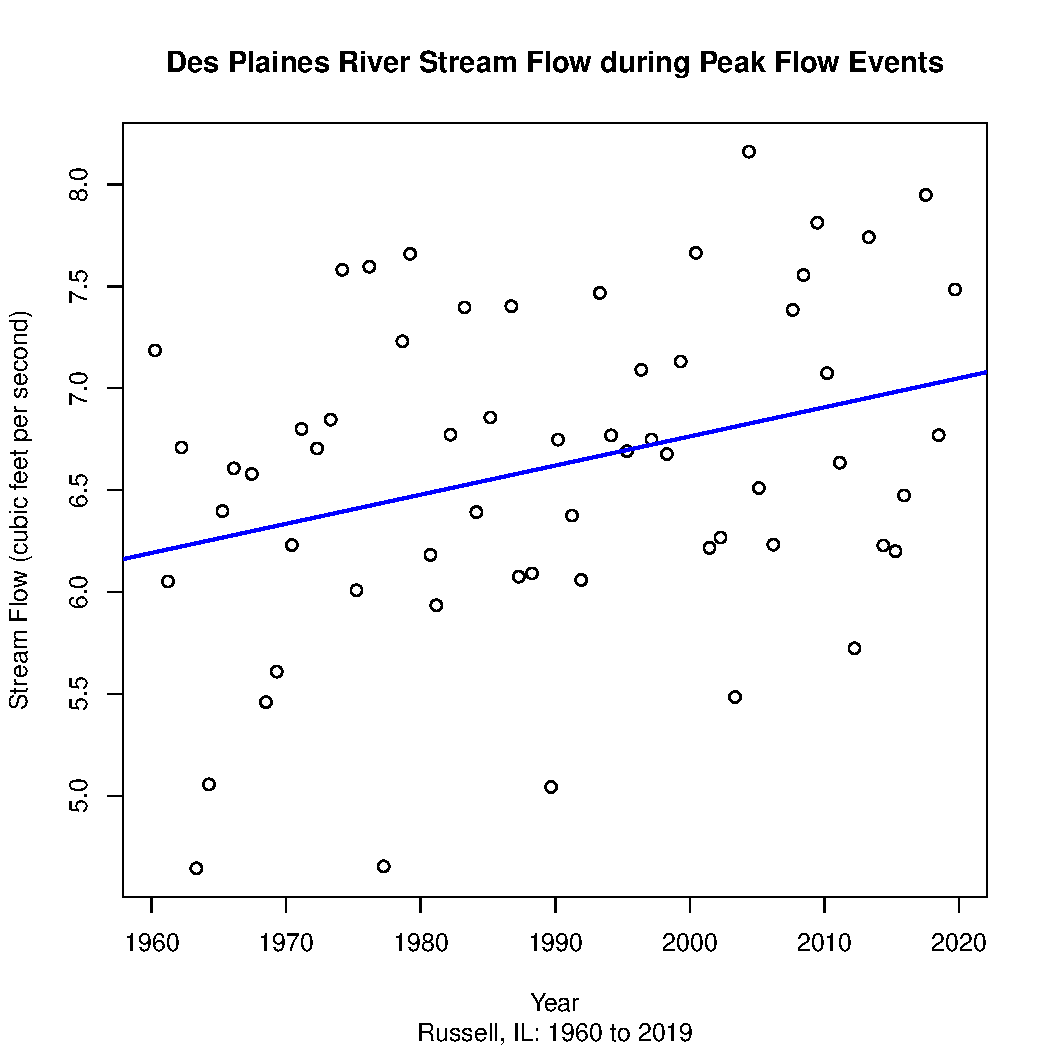
\includegraphics[width=\maxwidth]{figure/unnamed-chunk-1-1} 

\end{knitrout}

With a p-value of 0.016, I could comfortably reject the null hypothesis that there was no statistical evidence of a change in peak stream flow levels over time.  Although the correlation is low with an adjusted R-squared of 0.1 (meaning that approximately 10 percent of the variation in peak annual stream flow levels can be explained by the variation in the date), because natural phenomenon have so many conflicting variables I am satisfied with this level of correlation.  My hypothesis is complicated by the fact that the data does not meet the independence assumption necessary for linear modeling, because the data is taken in time-steps which are sequentially dependent.  However, the remaining assumption plots exhibit either minor or no trends, so I am comfortable moving forward with this analysis.

So, there is evidence that the volume of water flowing through the Des Plaines River during high water events had been increasing over half a century, even though there is limited evidence to suggest that precipitation levels have significantly changed over the same time period.  This leads to the question -- what HAS changed to result in the increasing streamflows during high flow events?  This could potentially have applications in land use change, as Lake County and the upstream regions have turned from agriculture to industry, and population has increased in the region over the past half the century.  This could imply more non-permeable surfaces, leading to a heavier dependence on the Des Plaines River.  More investigation is necessary to determine possible sources of this trend.
\end{document}
